\documentclass[tikz, border=10pt]{standalone}
\usetikzlibrary{positioning}
\usepackage{tkz-graph}
\begin{document}
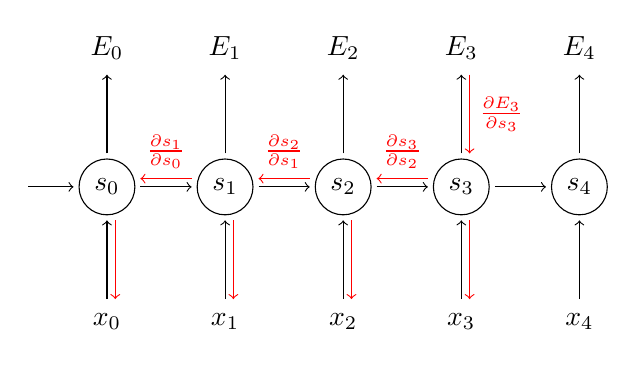
\begin{tikzpicture}

\newcommand \dd[2] {\frac{\partial #1}{\partial #2}} 
  
%  \node[outer sep=2] (equations) at (-2, 2) { 
%  	$s_t = \tanh(Ux_t + Ws_{t-1})$ \\
%	$o_t = \mathrm{softmax}(Vs_t)$
%	$L_t = y_{t} \log o_{t}$
%  };
  
  
    \foreach \t in {0,...,4} {
	\node[draw, outer sep=2, circle] (s\t) at (\t*1.5,0) {$s_\t$};
  	\node[outer sep=2] (x\t) [below=of s\t] {$x_\t$};
	\node[outer sep=2] (e\t) [above=of s\t] {$E_\t$};
	\path[->] (x\t) edge (s\t);
	\path[->] (s\t) edge (e\t);	
  }
  \path[->] (-1,0) edge (s0);
  
  \foreach \t in {0,...,3} {
  	\pgfmathtruncatemacro{\next}{\t + 1};
	\path[->] (s\t) edge (s\next);
  }
  
  % Draw derivatives
  \path[->, red] ([xshift=3] e3.south) edge  node[right] {\small $\dd{E_3}{s_3}$} ([xshift=3] s3.north);  
  \path[->, red] ([yshift=3] s3.west) edge node[above] {\small $\dd{s_3}{s_2}$} ([yshift=3] s2.east);
  \path[->, red] ([yshift=3] s2.west) edge node[above] {\small $\dd{s_2}{s_1}$} ([yshift=3] s1.east);
  \path[->, red] ([yshift=3] s1.west) edge node[above] {\small $\dd{s_1}{s_0}$} ([yshift=3] s0.east);
  \path[->, red] ([xshift=3] s3.south) edge ([xshift=3] x3.north);
  \path[->, red] ([xshift=3] s2.south) edge ([xshift=3] x2.north);
  \path[->, red] ([xshift=3] s1.south) edge ([xshift=3] x1.north);
  \path[->, red] ([xshift=3] s0.south) edge ([xshift=3] x0.north);

\end{tikzpicture}
\end{document}